\section{system model}
\begin{figure}[t]
\begin{center}
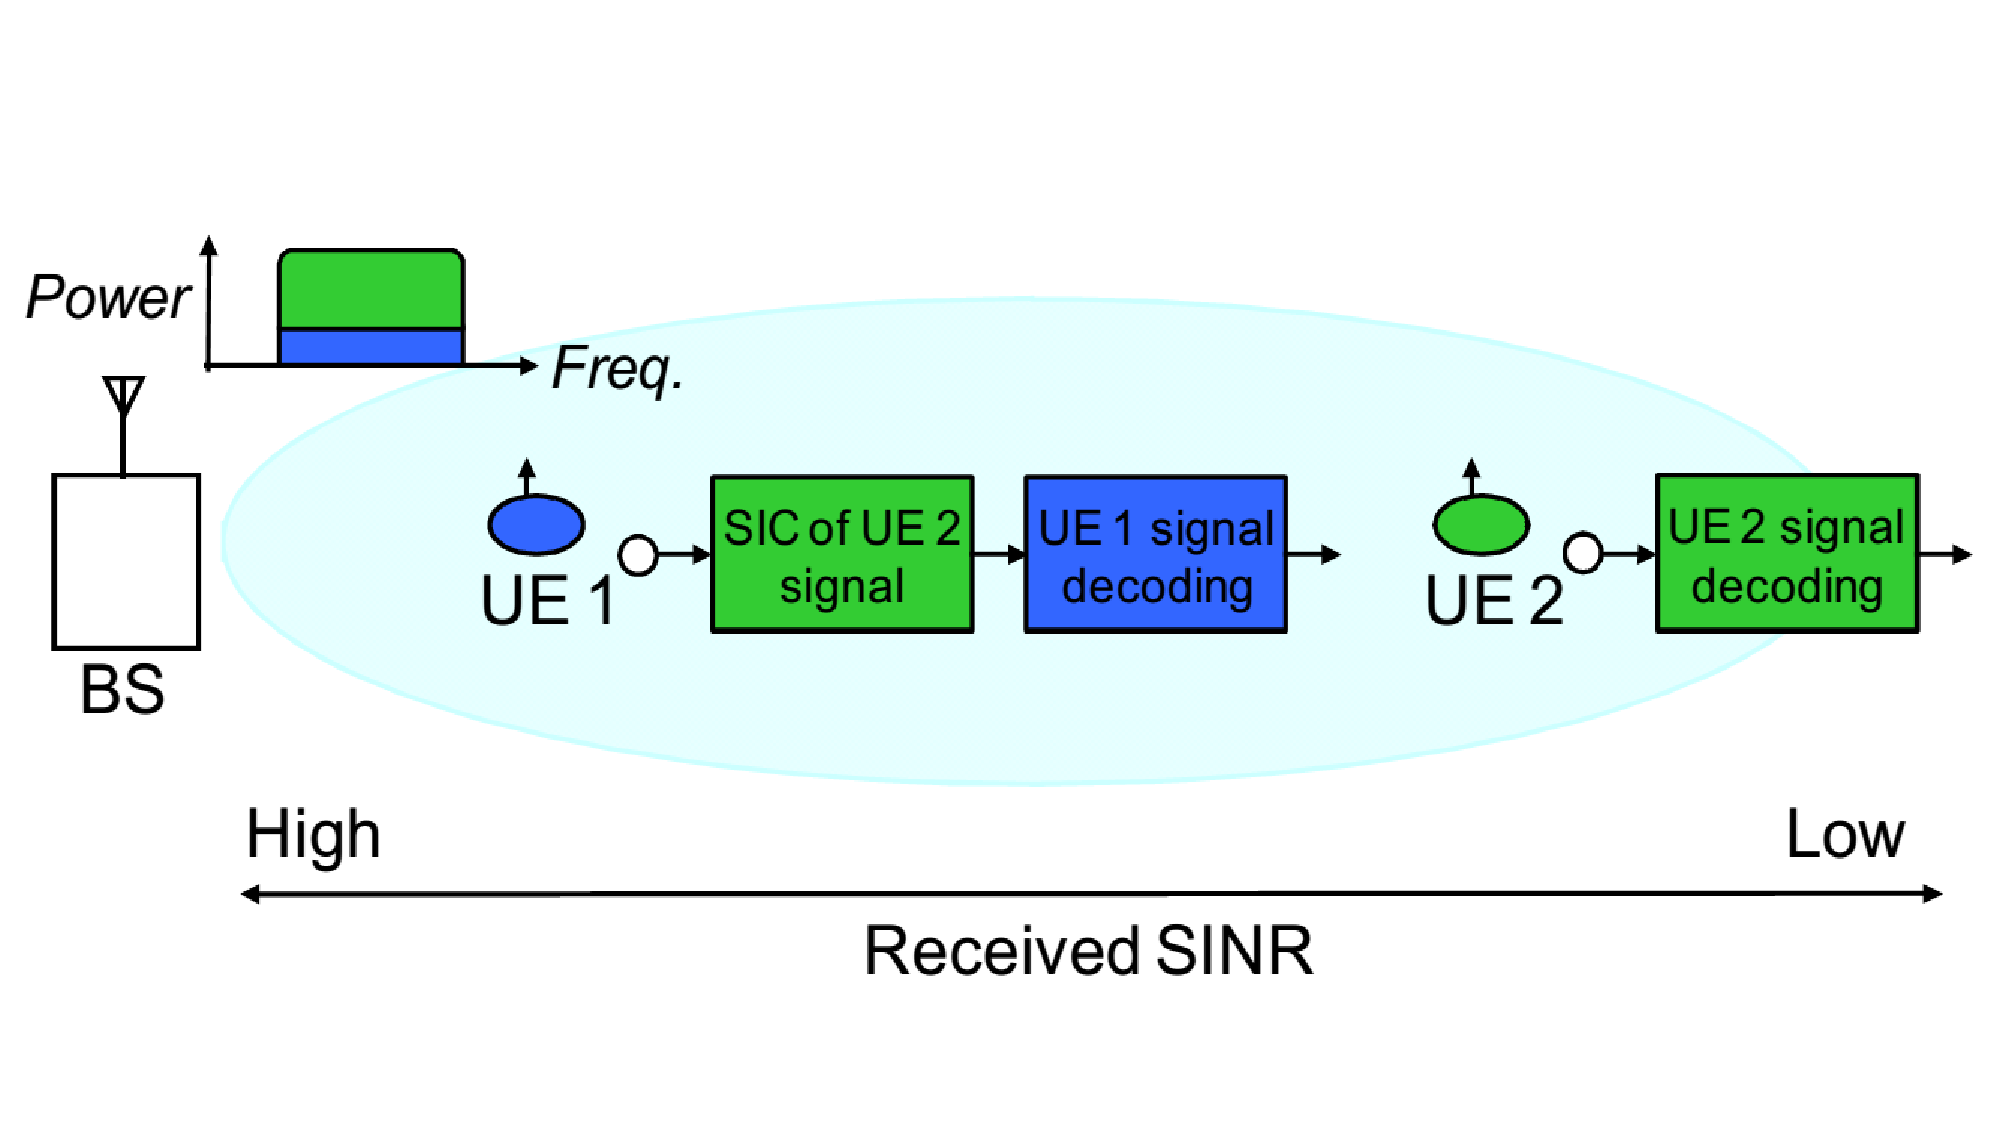
\includegraphics[width=1.0\columnwidth ,angle=0]{figure/NOMA_shannon}
\caption{Two-user SIC in the downlink}
\label{fig_NOMA_shannon}
\end{center}
\end{figure}
To understand how SIC works, take the two-user downlink communication in Fig.~\ref{fig_NOMA_shannon} as an example. The transmitted signal from the base station is a linear combination of the signals intended for UE1 and UE2. To decode individual signals, SIC needs to be performed at
each receiving UE. 
%In the NOMA downlink, the SIC process is implemented at the UE receiver. 
The optimal order for decoding is the order of the increasing channel gain normalized by the noise and inter-cell interference power. 
Assuming that the channel gain of UE1 is better than UE2, if UE2 can decode its signal, then UE1 must also be able to decode the UE2 signal.
Therefore, as shown in Fig.~\ref{fig_NOMA_shannon}, UE1 first decodes the signal of UE2 and then decodes its signal after the decoded
UE2 signal has been subtracted. 
%has to decode UE2's signal before decoding its signal, which is the concept of interference cancellation. 
For UE2, it can simply go ahead and decode its own signal without decoding the signal for UE1 first.
%However, UE2 does not perform interference cancellation. 
The case for SIC by $K$ UEs can be performed similarly, and ideally for any UE
the optimal decoding is to remove the interference coming from UEs with worse channel gains.
%, so (\ref{eq_sic_shannon}) is ideal interference cancellation.
As shown in~\cite{cite_docomo1}, 
the achievable rate $R_b^{\text{(sic)}}(k)$ for UE $k$ in resource $b$ can be represented as follows:
%accessing b-th resource and the k-th user throughput with SIC, , is represented as
\begin{equation}
\label{eq_sic_shannon}
R_b^{\text{(sic)}}(k)=W_b \text{log}_2 \left(1+\frac{|h_{k, b}|^2 P_{k, b}}{\displaystyle\sum^K_{{i=1} \atop {\frac{|h_{k, b}|^2}{N_{k, b}} < \frac{|h_{i, b}|^2}{N_{i, b}}}} |h_{k, b}|^2 P_{i, b} +W_b N_{k, b}} \right),
\end{equation}
where $|h_{i, b}|^2$ is channel gain between UE $i$ and the base station, $W_b$ is the bandwidth of resource $b$, $P_{i, b}$ is the transmission power allocated to UE $i$, and $N_{i, b}$ is the noise and inter-cell interference power for UE $i$.
% 分母中的sum是k沒有錯,指的是到第k-th user的i-th signal
Equation~\ref{eq_sic_shannon} shows a simple version of SIC reception model,
and the work in \cite{A_Successive_Interference_Cancellation_Scheme_for_an_OFDM_system}
investigate the design of a SISO SIC receiver operating on OFDM system
considering ICI cause by time variations in channel.
% fig
\begin{figure}[t]
\begin{center}
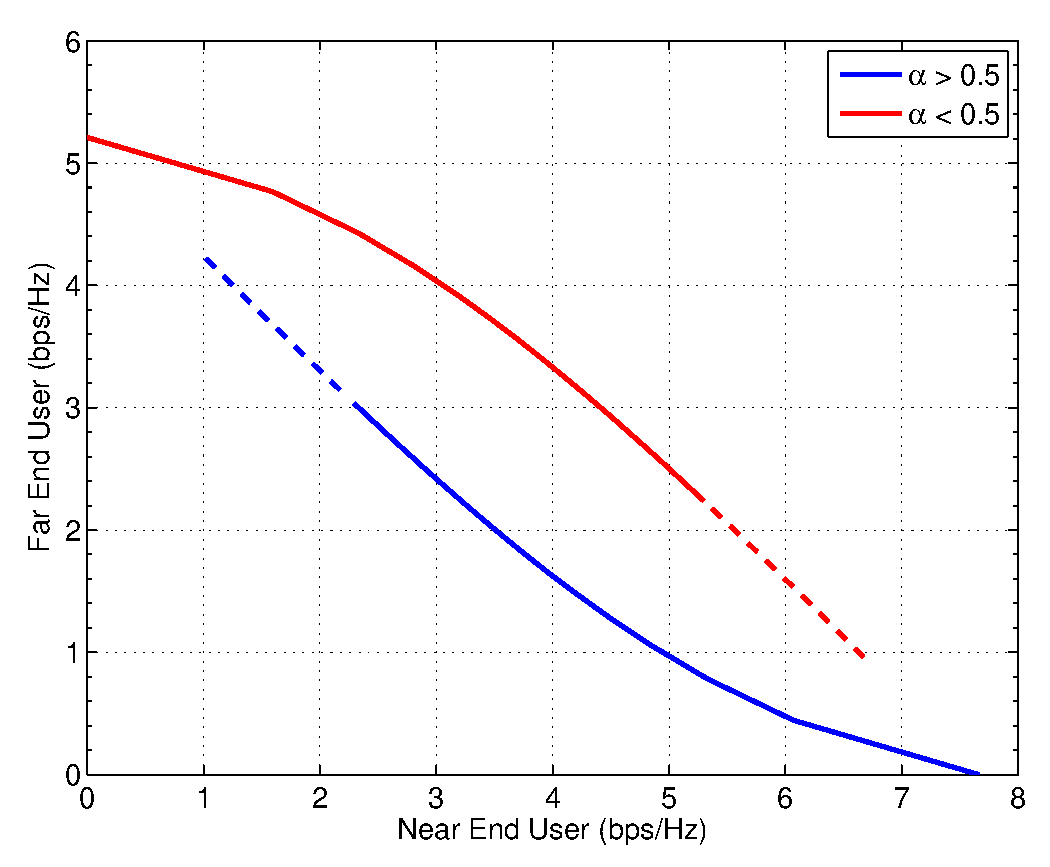
\includegraphics[width=0.95\columnwidth ,angle=0]{figure/u1VSu2.eps}
\caption{Upper boundary of rate in two users scheme}
\label{fig_ideal_r1r2}
\end{center}
\end{figure}
In the downlink scenario, the transmission power of the base station is limited
and denotes as $P$.
Assume there are two users that are served by the base station.
The power of the signal sent to near-end user, indexed as user 1, is $P_1=\alpha P$,
and far-end user, user 2, is $P_2=(1-\alpha)P$.
The channel is AWGN with pass loss exponent coefficient set to be $4.5$.
Consider the capture effect in receiving two signal in the same frequency, one with
stronger signal power will be demodulated. 
Thus as shown in Fig.~\ref{fig_ideal_r1r2}, when the power allocation factor $\alpha$
is greater than $0.5$, giving more power resource to near-end user, the curve is
convex. 
On the contrary, the curve is concave, which also indicates that there is
gain in weighted sum of throughputs.
The weighted sum rate \cite{cite_bell1} as a function of power allocation factor is 
defined as follows,
\begin{equation}
\label{eq_sic_weighted_sum_rate}
Gain = \frac{1}{R_1(P)}R_1(\alpha P) + \frac{1}{R_2(P)}R_2((1-\alpha)P)
\end{equation}
where $R_1$, $R_2$ are functions denotes channel capacity with given power allocated.
The measure for the system performance is enhanced by weighted sum rate, since optimizing
the sum rate of all users in the system results in serving specific user with good channel
condition.
% fig
\begin{figure}[t]
\begin{center}
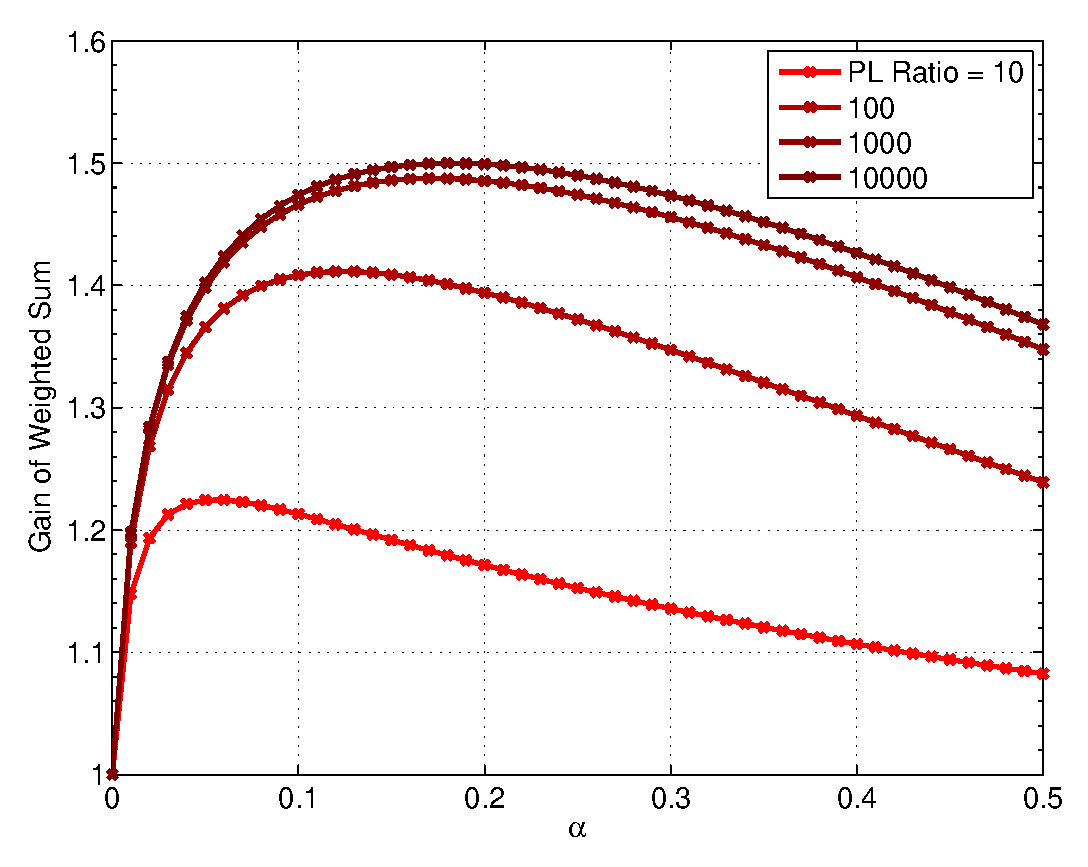
\includegraphics[width=1.0\columnwidth ,angle=0]{figure/alphaVSgain.eps}
\caption{Gain in Weighted sum of throughput for different PL ratio}
\label{fig_ideal_gain}
\end{center}
\end{figure}
In Fig.~\ref{fig_ideal_gain} the gain in weighed sum changes by different power allocation 
factor selected, and an optimal allocation varies for different pass loss ratio of user 1
and user 2.
As the difference of the PL ratio increase the gain in weighted sum increase also.
However, we've observed that the maximum of the gain is limited and possibly converges.
